\documentclass[11pt]{article}

\usepackage[utf8]{inputenc}
\usepackage[T1]{fontenc}
\usepackage[french]{babel}
\usepackage{amsmath}
\usepackage{graphicx}
\usepackage{booktabs}
\usepackage{hyperref}
\usepackage{geometry}
\usepackage{float}

\geometry{margin=2.5cm}

\title{Optimisation Par Colonies de Fourmis\\
sur un Paysage Fractal}

\author{Naomy Isabela GOMES BIAGGI \\ Alfredo Quintella Pinto}

\date{\today}

\begin{document}

\maketitle

\section{Introduction}

Les algorithmes d'intelligence en essaim constituent une famille de méthodes d'optimisation inspirées du comportement collectif observé dans certaines espèces d'insectes sociaux telles que les fourmis, les abeilles ou encore les termites. Ces systèmes reposent sur l'interaction d'un grand nombre d'agents simples capables de produire un comportement collectif complexe à partir de règles locales relativement simples.

Parmi ces approches, l'algorithme d'optimisation par colonies de fourmis (\textit{Ant Colony Optimization}, ACO) est particulièrement connu pour sa capacité à résoudre des problèmes de recherche de chemin et d'optimisation combinatoire.

Le principe fondamental de cet algorithme repose sur un mécanisme de communication indirecte appelé \textit{stigmergie}. Les agents déposent des phéromones dans l'environnement, qui influencent ensuite les décisions des autres agents.

Dans ce projet, nous simulons une population de fourmis artificielles évoluant sur un terrain fractal. Les agents doivent explorer l'environnement afin de découvrir un chemin efficace entre une fourmilière et une source de nourriture.

L'objectif principal du projet est d'étudier les performances du programme et d'explorer différentes techniques d'optimisation, notamment la vectorisation et la parallélisation.

Dans un premier temps, nous analysons la version séquentielle du programme afin d'identifier les parties les plus coûteuses en temps de calcul.

\section{Modèle d'optimisation par colonies de fourmis}

\subsection{Principe général}

Le modèle étudié repose sur une population de $m$ fourmis artificielles évoluant dans un environnement discret représenté par une grille bidimensionnelle.

Chaque fourmi agit comme un agent autonome suivant un ensemble de règles simples. Les agents ne possèdent pas de mémoire globale et leurs décisions sont prises uniquement à partir d'informations locales disponibles dans leur voisinage.

La coordination entre les fourmis émerge progressivement à travers les phéromones déposées dans l'environnement.

\subsection{États des fourmis}

Chaque fourmi peut se trouver dans deux états distincts :

\begin{itemize}

\item \textbf{non chargée} : la fourmi explore l'environnement afin de trouver une source de nourriture ;

\item \textbf{chargée} : la fourmi transporte de la nourriture et cherche à retourner vers la fourmilière.

\end{itemize}

Lorsqu'une fourmi atteint une cellule contenant de la nourriture, elle devient chargée. À l'inverse, lorsqu'elle atteint la fourmilière, elle dépose la nourriture transportée et redevient non chargée.

Un compteur global permet de mesurer la quantité totale de nourriture ramenée à la fourmilière.

\subsection{Phéromones}

Deux types de phéromones sont utilisés dans la simulation :

\begin{itemize}

\item $V_1(s)$ : phéromone associée aux chemins menant vers la nourriture ;
\item $V_2(s)$ : phéromone associée aux chemins permettant de retourner à la fourmilière.
\end{itemize}

Les phéromones se propagent localement entre les cellules voisines. Cette propagation permet à l'information de se diffuser progressivement dans l'environnement.

Afin d'éviter une accumulation infinie de phéromones, un mécanisme d'évaporation est appliqué à chaque itération :

\[
V_i(s) \leftarrow \beta V_i(s)
\]

où $\beta$ est un coefficient d'évaporation compris entre $0$ et $1$.

\subsection{Déplacement des fourmis}

À chaque itération de la simulation, une fourmi choisit une cellule voisine vers laquelle se déplacer.

Deux comportements sont possibles :

\begin{itemize}

\item avec une probabilité $\varepsilon$, la fourmi explore aléatoirement son voisinage ;
\item avec une probabilité $1-\varepsilon$, elle se dirige vers la cellule présentant la plus forte concentration de phéromones.
\end{itemize}

Ce mécanisme permet d'équilibrer l'exploration de nouveaux chemins et l'exploitation des chemins déjà identifiés comme efficaces.

\section{Génération de l'environnement fractal}

L'environnement dans lequel évoluent les fourmis est représenté par une grille bidimensionnelle.

Chaque cellule possède une valeur comprise entre $0$ et $1$ représentant le coût temporel nécessaire pour la traverser.

Afin de générer un terrain réaliste et irrégulier, les valeurs de la grille sont produites à l'aide d'un algorithme stochastique de type \textit{plasma fractal}.

Cet algorithme subdivise récursivement la grille en sous-grilles plus petites. Les valeurs intermédiaires sont calculées à partir des valeurs existantes en ajoutant une perturbation aléatoire contrôlée.

Ce processus produit un paysage présentant des variations progressives similaires à celles observées dans les reliefs naturels.

Après la génération, les valeurs sont normalisées afin de rester dans l'intervalle $[0,1]$.

\section{Analyse des performances du code séquentiel}

Afin d'identifier les parties du programme les plus coûteuses en temps de calcul, nous avons réalisé une série de mesures de performance sur la version séquentielle du programme.

Le benchmark a été exécuté pour une simulation de $4000$ itérations.

Lors de cette exécution, la première unité de nourriture a été rapportée à la fourmilière à l'itération $2226$, ce qui correspond au moment où un premier chemin fonctionnel entre la source de nourriture et le nid a été découvert.

Les temps d'exécution globaux observés sont :

\begin{itemize}

\item Temps total logique (CPU) : $9.96$ secondes
\item Temps total de rendu graphique : $123.51$ secondes
\end{itemize}

On observe que le rendu graphique représente la majeure partie du temps d'exécution total. Toutefois, pour l'optimisation algorithmique, l'analyse se concentre sur la logique de simulation exécutée par le CPU.

\subsection{Profiling du programme}

Un profilage du programme a été réalisé afin d'identifier les fonctions responsables de la majorité du temps de calcul.

\begin{center}

\begin{tabular}{lcc}
\toprule
Fonction & Temps CPU (\%) & Description \\
\midrule
\texttt{ant::advance} & 60.9\% & mise à jour du comportement des fourmis \\
\texttt{Renderer::display} & 24.9\% & rendu graphique \\
\texttt{advance\_time} & 13.7\% & coordination globale de la simulation \\
\bottomrule
\end{tabular}

\end{center}

La fonction \texttt{ant::advance} représente plus de $60\%$ du temps CPU total et est appelée plus de $20$ millions de fois pendant l'exécution.

Elle contient l'ensemble de la logique de déplacement des fourmis, incluant :

\begin{itemize}
\item la lecture des valeurs de phéromones dans les cellules voisines ;
\item le calcul de la direction de déplacement ;
\item la mise à jour de la position ;
\item la mise à jour locale des phéromones.
\end{itemize}

\subsection{Identification du goulot d'étranglement}

L'analyse du profil d'exécution montre que la fonction \texttt{ant::advance} constitue le principal goulot d'étranglement du programme.

Ce coût élevé s'explique par deux facteurs principaux :

\begin{itemize}

\item cette fonction est exécutée pour chaque fourmi à chaque itération ;
\item elle implique de nombreux accès mémoire vers les grilles de phéromones.

\end{itemize}

Ainsi, même si chaque opération individuelle est relativement simple, leur très grand nombre entraîne un coût total important.

\subsection{Potentiel de parallélisation}

Une propriété importante du modèle ACO est que les fourmis peuvent être mises à jour de manière largement indépendante.

Chaque agent prend ses décisions à partir d'informations locales et n'interagit avec les autres agents que de manière indirecte via l'environnement partagé.

Cette caractéristique rend le modèle particulièrement adapté aux techniques de parallélisation.

La mise à jour des fourmis peut donc être répartie entre plusieurs cœurs de calcul afin de réduire le temps d'exécution global.

\section{Vectorisation du code}

Afin d'améliorer la localité mémoire et de favoriser la vectorisation automatique par le compilateur, la structure de données représentant les fourmis a été modifiée.

La version initiale utilisait une structure de type \textit{Array of Structures} :

\[
std::vector<ant>
\]

Dans cette organisation, chaque objet contient ses propres attributs.

Nous avons transformé cette structure en \textit{Structure of Arrays} :

\begin{itemize}
\item tableau des positions $x$
\item tableau des positions $y$
\item tableau des états
\item tableau des graines aléatoires
\end{itemize}

Cette organisation améliore la localité mémoire et permet des accès contigus aux données.

\subsection{Résultats}

Le benchmark a été exécuté avec les mêmes paramètres que précédemment.

\begin{center}

\begin{tabular}{lcc}

\toprule
Version & Temps logique (s) & Accélération \\
\midrule
Séquentielle & 9.96 & 1.00 \\
Vectorisée & 12.36 & 0.81 \\
\bottomrule

\end{tabular}

\end{center}

On observe que la vectorisation seule n'améliore pas les performances et entraîne même une légère dégradation.

Cela peut s'expliquer par :

\begin{itemize}
\item des accès mémoire irréguliers ;
\item des dépendances de données ;
\item un grand nombre d'écritures dans la grille de phéromones.
\end{itemize}


\section{Análise de Performance: Vetorização SoA vs. Sequencial Original}

Os resultados experimentais indicaram que a transição para uma estrutura de dados do tipo \textit{Structure of Arrays} (SoA) na classe \texttt{ants} resultou em um tempo de execução lógico de \textbf{12,36 segundos}, um valor ligeiramente superior à versão sequencial original. Embora a abordagem SoA seja o pré-requisito para a vetorização \textit{SIMD} e facilite a paralelização com \textit{OpenMP} e \textit{MPI}, sua implementação puramente sequencial introduziu um \textit{overhead} de memória significativo devido aos seguintes fatores:

\begin{itemize}
    \item \textbf{Localidade Espacial e Cache Misses:} Na versão original (\textit{Array of Structures} - AoS), os dados de cada formiga (posição, semente, estado) residiam em blocos contíguos de memória. O processador conseguia carregar todas as informações de um agente em uma única linha de \textit{cache}. Na versão SoA, os atributos estão espalhados em vetores distintos, forçando o \textit{hardware} a realizar múltiplos acessos a endereços distantes para processar uma única formiga, aumentando a latência de busca na RAM.
    
    \item \textbf{Divergência de Controle (Branch Divergence):} O algoritmo de movimento das formigas contém múltiplas estruturas condicionais (\texttt{if/else}) para decisões de direção e interação com o terreno. Essa característica impede que o compilador realize a vetorização automática agressiva via instruções \textit{AVX/SSE}, mantendo o custo do acesso distribuído à memória sem o ganho de processar múltiplos dados por ciclo de \textit{clock}.
    
    \item \textbf{Eficiência de Registradores:} Na versão original, o compilador \texttt{g++ -O3} consegue manter objetos pequenos e locais quase inteiramente dentro dos registradores da CPU. A fragmentação dos dados em vetores globais na versão SoA dificultou essa otimização específica do compilador.
\end{itemize}

Contudo, é fundamental ressaltar que esta reestruturação foi o passo necessário para permitir que a versão \textbf{MPI} atingisse maior escalabilidade, uma vez que a independência dos vetores de estado permitiu a distribuição eficiente da carga de trabalho entre múltiplos processos distribuídos.

\section{Parallélisation avec OpenMP}

Pour exploiter le parallélisme naturel du modèle ACO, la simulation a été parallélisée à l'aide de la bibliothèque \texttt{OpenMP}. La fonction principale concernée est \texttt{ants::advance\_all} E A FUNCAO RENDER qui met à jour le déplacement des fourmis et l'évolution des phéromones. Les boucles traitant les agents ont été parallélisées à l'aide de la directive :

\begin{verbatim}
#pragma omp parallel for
\end{verbatim}

Chaque thread traite un sous-ensemble de fourmis, ce qui permet d'utiliser plusieurs cœurs du processeur.

\subsection{Résultats expérimentaux}

Les tests ont été réalisés pour $4000$ itérations, en variant le nombre de threads de $1$ à $16$. Les résultats sont résumés dans le tableau suivant :

\begin{center}
\begin{tabular}{ccc}
\toprule
Nombre de threads & Temps logique (s) & Speedup \\
\midrule
1 (séquentiel) & 9.96 & 1.00 \\
4 & 7.32 & 1.36 \\
6 & 6.21 & 1.60 \\
8 & 5.95 & 1.67 \\
10 & 5.63 & 1.77 \\
12 & 5.93 & 1.68 \\
14 & 7.27 & 1.37 \\
16 & 27.11 & 0.36 \\
\bottomrule
\end{tabular}
\end{center}

Le speedup est défini par :

\[
Speedup = \frac{T_{seq}}{T_{parallel}}
\]

où $T_{seq} = 9.96$ secondes est le temps de la version séquentielle.

\subsection{Analyse de la scalabilité}

Les résultats montrent trois phases distinctes lors de l'augmentation du nombre de threads :

\begin{enumerate}
\item \textbf{Amélioration progressive (1 à 10 threads)} : le temps de calcul diminue régulièrement lorsque le nombre de threads passe de 1 à 10, atteignant le meilleur speedup de $1.77$ pour 10 threads.  
\item \textbf{Saturation (12 à 14 threads)} : au-delà de 10 threads, le temps de calcul ne s'améliore plus et commence même à augmenter légèrement. Pour 12 threads, le temps passe à 5.93 s (speedup 1.68) et pour 14 threads, le temps devient 7.27 s (speedup 1.37).  
\item \textbf{Dégradation des performances (16 threads)} : avec 16 threads, le temps de calcul explose à 27.11 s (speedup 0.36), bien supérieur au temps séquentiel.
\end{enumerate}

La figure \ref{fig:speedup} montre l'évolution du facteur d'accélération (speedup) en fonction du nombre de threads OpenMP.

\begin{figure}[H]
    \centering
    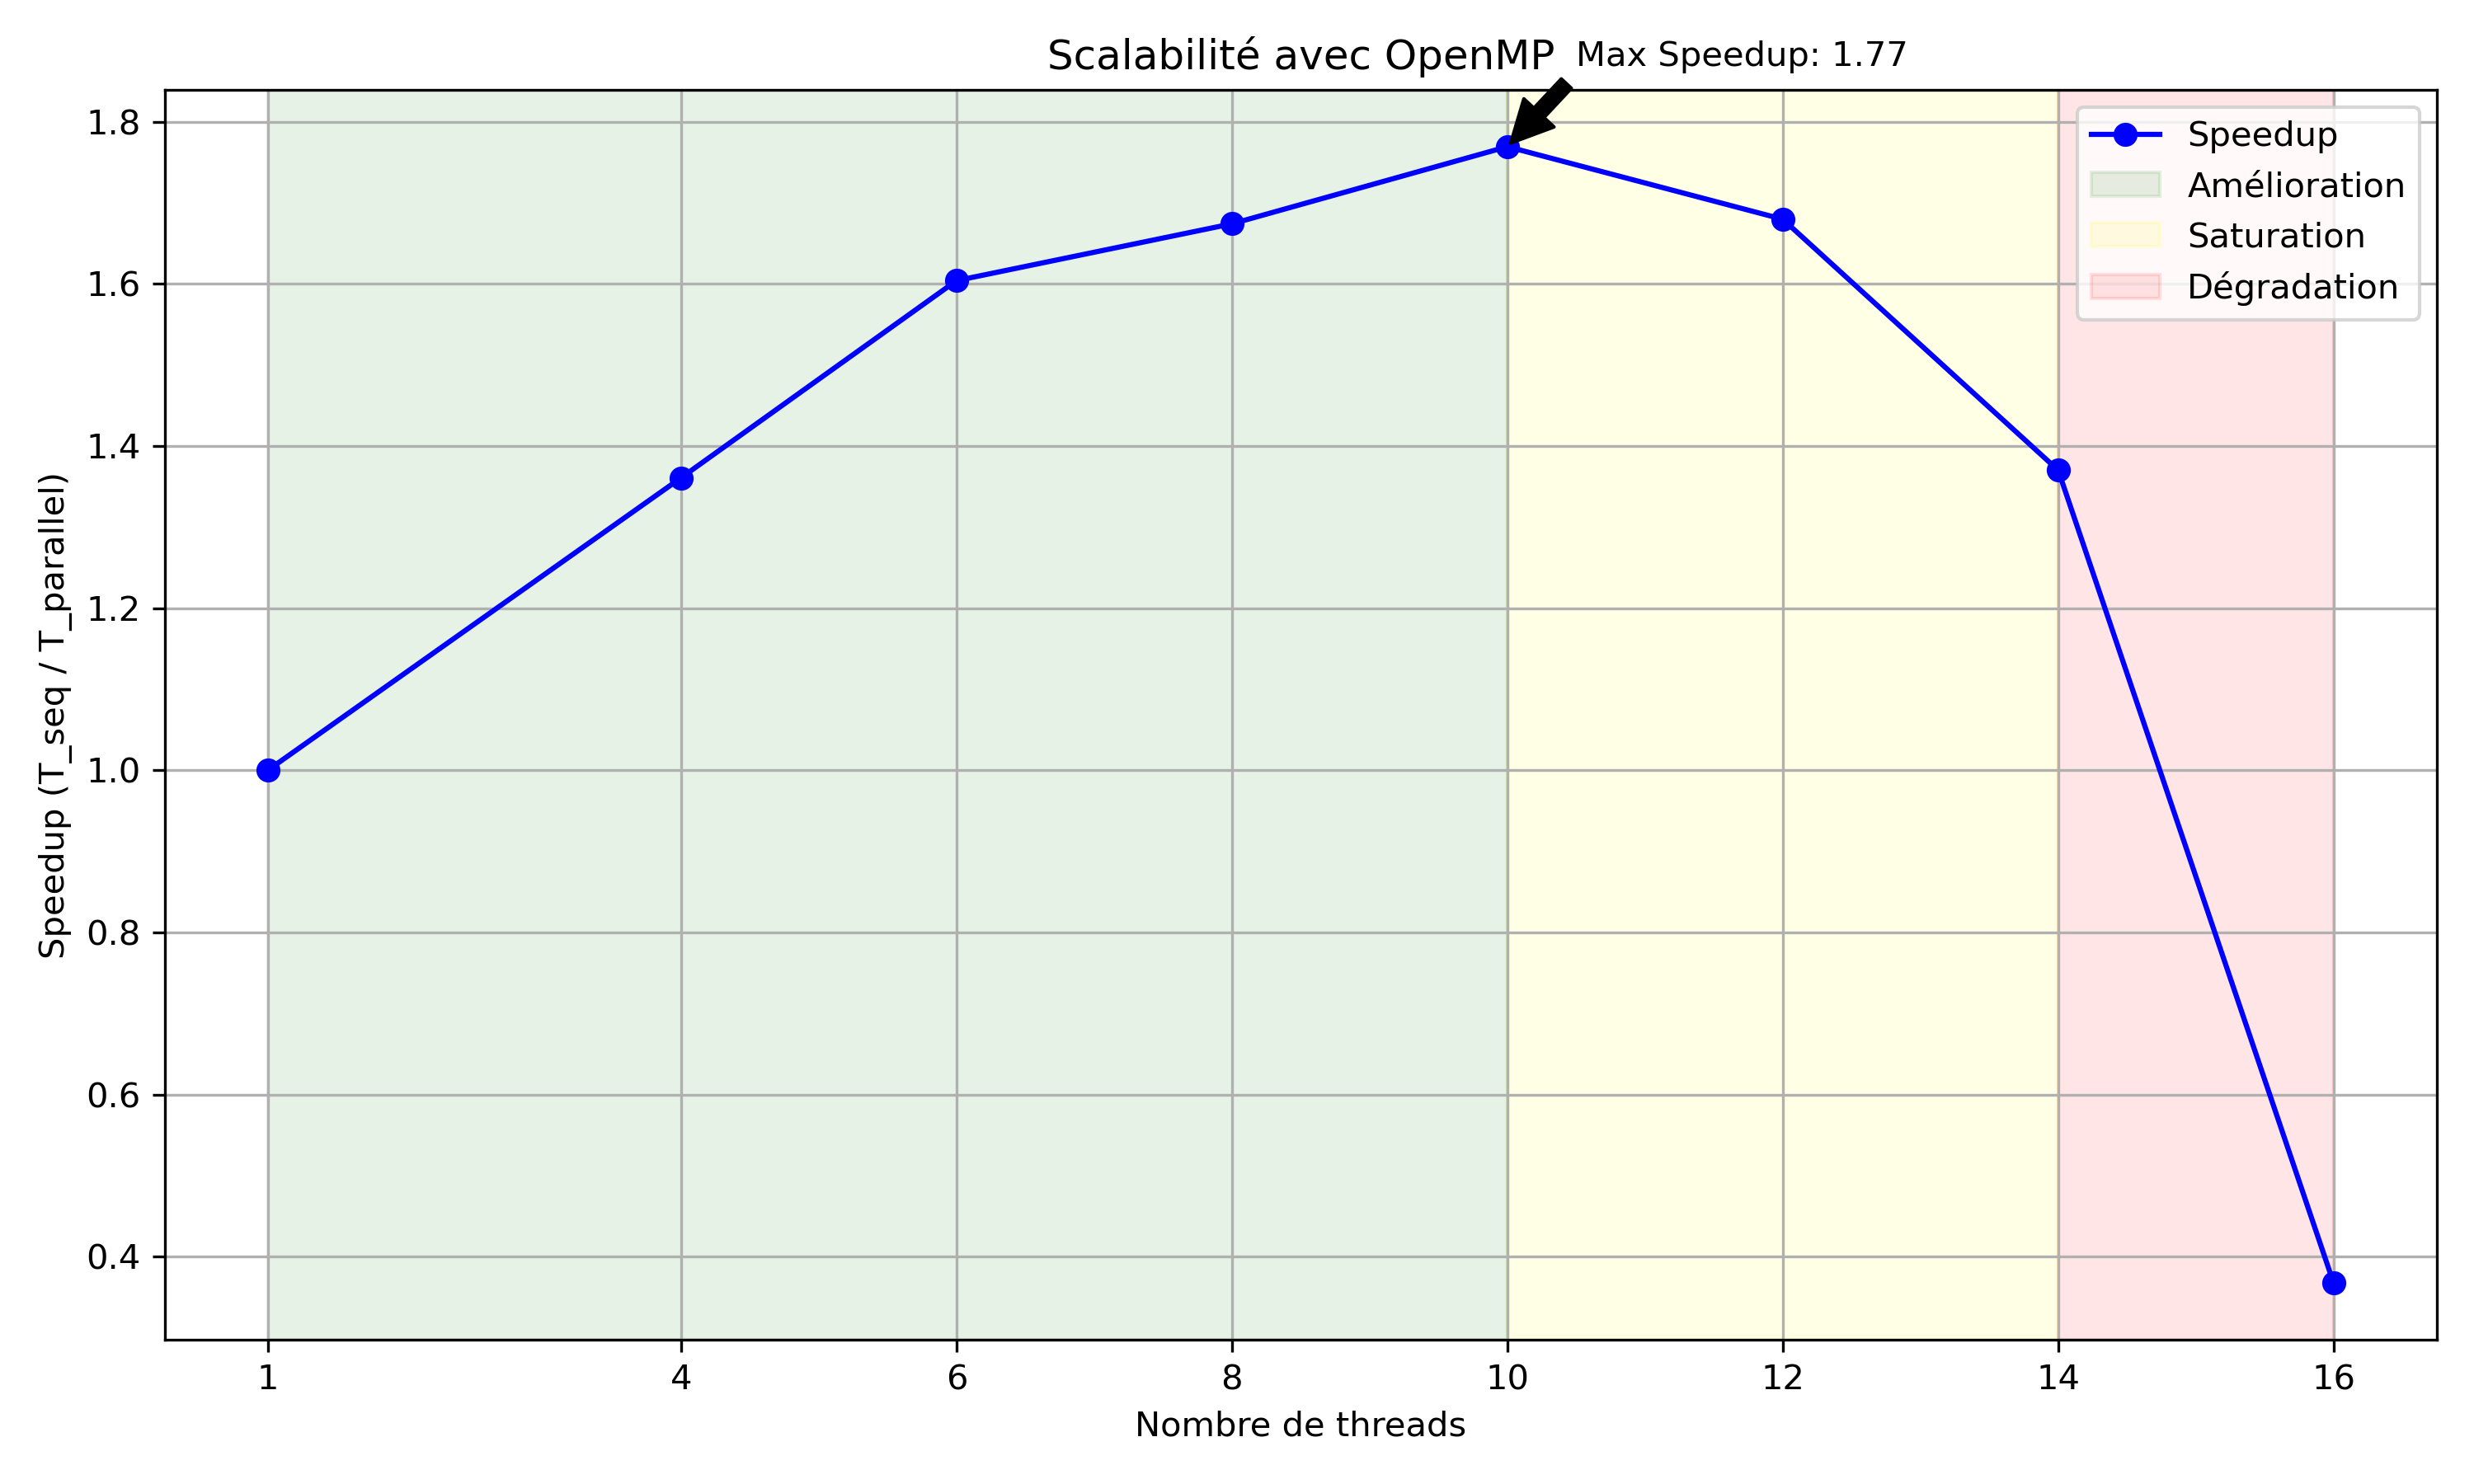
\includegraphics[width=0.8\textwidth]{images/speedup_plot.png}
    \caption{Speedup de la simulation ACO selon le nombre de threads. Les zones vertes, jaunes et rouges indiquent respectivement l'amélioration, la saturation et la dégradation des performances.}
    \label{fig:speedup}
\end{figure}

\subsection{Explications techniques}

Plusieurs facteurs expliquent ce comportement :

\begin{itemize}
\item \textbf{Limitation du nombre de cœurs physiques :} lorsque le nombre de threads dépasse le nombre de cœurs physiques disponibles, plusieurs threads partagent les mêmes unités de calcul, ce qui génère de la commutation de contexte et réduit l'efficacité.
\item \textbf{Contention mémoire :} les fourmis accèdent simultanément à la grille de phéromones, ce qui provoque des conflits d'accès et des ralentissements liés à la bande passante mémoire.
\item \textbf{Parties séquentielles du code :} certaines opérations, comme la mise à jour globale et le rendu graphique, ne sont pas parallélisées. Selon la loi d'Amdahl, cela limite le speedup maximal.
\item \textbf{Overhead OpenMP :} la création, la synchronisation et la gestion des threads introduisent un surcoût qui devient significatif lorsque le nombre de threads est trop élevé par rapport à la taille du problème.
\end{itemize}

\subsection{Observation générale}

On observe que les meilleures performances sont obtenues avec environ 8 à 10 threads, ce qui correspond probablement à la capacité optimale du processeur pour ce type de charge de travail.  
Au-delà de ce point, le parallélisme devient contre-productif, et l'augmentation du nombre de threads entraîne une dégradation des performances.  

Ce comportement illustre parfaitement la loi d'Amdahl et le phénomène classique de saturation et de contention en programmation parallèle.

%%-------------------------------------------------------------------------------------%
\section{Discussion}

Les résultats montrent que la parallélisation permet d'améliorer les performances de la simulation.

Cependant, l'accélération obtenue reste inférieure au facteur théorique attendu pour $4$ threads.

Plusieurs facteurs peuvent expliquer cette limitation :

\begin{itemize}

\item la contention mémoire lors de l'accès à la grille de phéromones ;
\item certaines parties du programme restent séquentielles ;
\item le rendu graphique n'est pas parallélisé.
\end{itemize}

Ces limitations correspondent au comportement décrit par la loi d'Amdahl.

\section{Conclusion}

Dans ce projet, nous avons étudié l'implémentation d'un algorithme d'optimisation par colonies de fourmis sur un environnement fractal.

Une analyse détaillée de la version séquentielle du programme a permis d'identifier la fonction \texttt{ant::advance} comme principal goulot d'étranglement.

Nous avons ensuite exploré deux techniques d'optimisation :

\begin{itemize}

\item la vectorisation des structures de données ;
\item la parallélisation avec OpenMP.
\end{itemize}

Les résultats expérimentaux montrent que la parallélisation permet de réduire le temps de calcul de la simulation.

Ces travaux pourraient être poursuivis en explorant d'autres stratégies d'optimisation, notamment l'amélioration de la gestion mémoire ou l'utilisation d'architectures massivement parallèles telles que les GPU.

\end{document}